%%%%%%%%%%%%%%%%%%%%%%%%%%%%%%%%%%%%%%%%%%%%%%%%%%%%%%%%%%%%%%%%%%%%%%%%%%%%%%%%%%%%%%%%%%%%%%%%%%%%%%%%%%%%%%%%%%%%%%%%%%%%%%%%%%%%%%%%%%%%%%%%%%%%%%%%%%%
% This is just an example/guide for you to refer to when submitting manuscripts to Frontiers, it is not mandatory to use Frontiers .cls files nor frontiers.tex  %
% This will only generate the Manuscript, the final article will be typeset by Frontiers after acceptance.   
%                                              %
%                                                                                                                                                         %
% When submitting your files, remember to upload this *tex file, the pdf generated with it, the *bib file (if bibliography is not within the *tex) and all the figures.
%%%%%%%%%%%%%%%%%%%%%%%%%%%%%%%%%%%%%%%%%%%%%%%%%%%%%%%%%%%%%%%%%%%%%%%%%%%%%%%%%%%%%%%%%%%%%%%%%%%%%%%%%%%%%%%%%%%%%%%%%%%%%%%%%%%%%%%%%%%%%%%%%%%%%%%%%%%

%%% Version 3.4 Generated 2018/06/15 %%%

\documentclass[utf8, a4paper, final, crop]{frontiersSCNS}
\usepackage[switch]{lineno} %   columnwise

\usepackage{url,lineno,microtype,subcaption}


\usepackage[onehalfspacing]{setspace}

\usepackage{fontspec} 
\setmainfont[Mapping=tex-text]{Times New Roman}

\usepackage{minted}  % for styling python code
\newcommand{\pythoninline}[1]{\mintinline{python}{#1}}
\newcommand{\bashinline}[1]{\mintinline{bash}{#1}}

\usepackage[british]{babel}
\hyphenation{projects-mouselemuratlas}

\usepackage{hyperref}
\hypersetup{
  colorlinks   = true, %Colours links instead of ugly boxes
  urlcolor     = blue, %Colour for external hyperlinks
  linkcolor    = blue, %Colour of internal links
  citecolor    = red, %Colour of citations
  filecolor	   = magenta,      
  pdftitle	   = {Sammba-MRI},
  bookmarks    = true
}

\usepackage{soul} % highlight changes
\usepackage{cancel} % strike through text
\newcommand\Ccancel[1]{\renewcommand\CancelColor{\color{red}}\xcancel{#1}}

\linenumbers

\def\keyFont{\fontsize{8}{11}\helveticabold }
\def\firstAuthorLast{Bougacha {et~al.}}
\def\Authors{Salma Bougacha\,$^{1,2,3,4}$, Nachiket A. Nadkarni\,$^{1,2}$, 
Marina Celestine\,$^{1,2}$, Cl\'ement M. Garin\,$^{1,2}$, and Marc 
Dhenain\,$^{1,2,*}$}

\def\Address{$^{1}$UMR9199 Laboratory of Neurodegenerative Diseases Mechanisms, Centre National de la Recherche Scientifique (CNRS), Fontenay-aux-Roses, France

$^{2}$MIRCen, Institut Fran\c{c}ois Jacob, Commissariat \`a l'Energie Atomique et aux Energies Alternatives (CEA), Fontenay aux Roses, France 

$^{3}$UMR-S U1237 Physiopathologie et imagerie des troubles Neurologiques (PhIND), INSERM, Universit\'e de Caen-Normandie, GIP Cyceron, Caen, France 

$^{4}$Normandie Universit\'e, UNICAEN, PSL Research University, EPHE, Inserm, U1077, CHU de Caen, Neuropsychologie et Imagerie de la M\'emoire Humaine, Caen, France
}

\def\corrAuthor{Marc Dhenain, MIRCen, UMR CEA-CNRS 9199, 18 Route du Panorama,92265 Fontenay-aux-Roses CEDEX, France}

\def\corrEmail{marc.dhenain@cea.fr}

\begin{document}
\setstcolor{red}  % color for striking through text

\firstpage{1}

\title[Sammba-MRI]{Sammba-MRI: a library for processing SmAll MaMmals BrAin MRI data in Python} 


\author[\firstAuthorLast ]{\Authors} %This field will be automatically populated
\address{} %This field will be automatically populated
\correspondance{} %This field will be automatically populated

\extraAuth{}

\maketitle

\begin{abstract}

Small mammals neuroimaging offers incredible opportunities to investigate structural and
functional aspects of the brain. Many tools have been developed in the last decade to analyse
small animal data, but current software\Ccancel{s} are less mature than the available tools that process
human brain data. The Python package Sammba-MRI (SmAll MaMmals BrAin MRI in Python;
\url{http://sammba-mri.github.io}) is designed to allow flexible and efficient use of existing methods and
enables fluent scriptable analysis workflows, from raw data conversion to multimodal
processing.

\tiny
 \keyFont{ \section{Keywords:} Processing pipeline, MRI, registration, small animal Neuroimaging, Python } 

\end{abstract}

\section{Introduction}

The use of magnetic resonance imaging (MRI) methods in animals
provides considerable benefits for improving our understanding
of the brain structure and functioning in health and disease.
The greatest advantages of preclinical MRI include
group homogeneity and the opportunity to acquire a high amount of information
repeated or modulated as needed.
This added value, together with practical and ethical considerations,
resulted in an increase of the use of small mammals MRI in research.
However, while human brain imaging benefits from a large variety of high 
level software solutions 
for MRI preprocessing and analysis, preclinical MRI
is left behind.
There is currently an urgent need for
efficient and collaborative tools that would facilitate the adoption and 
dissemination of standardized pre-processing strategies for small animal MRI.

\section{Tools: Python ecosystem and neuroimaging software packages}

With its Free and Open Source Software (FOSS)
dependency stack and its growing neuroimaging community 
Python has been naturally the language of choice for our
package.
The scientific Python libraries used in Sammba-MRI are
NumPy \citep{oliphant2006guide}, SciPy \citep{millman2011python}, the neuroimaging 
data analysis tools nibabel\footnote{\url{https://nipy.org/nibabel/}}, Nilearn \citep{abraham2014machine} and 
Nipype \citep{gorgolewski2011Nipype}.
Visualization functionality depends on Matplotlib \citep{hunter2007matplotlib} 
or Graphviz \citep{gansner2000open}, but neither is required to perform
MRI data processing.

Via Nipype, we utilize basic MRI preprocessing
functions from AFNI \citep{cox1996afni}, FSL \citep{jenkinson2012fsl} and ANTs 
\citep{avants2009advanced}
packages. The dependency on the efficient but non open-source brain segmentation RATs 
tool \citep{oguz2014rats} is optional.

\section{Code design}

Coding guidelines follow the
model of Nilearn and other successfully adopted packages
\citep[e.g. Scikit-learn][]{pedregosa2011scikit} 
to make the codebase understandable and easily maintainable\footnote{\url{http://gael-varoquaux.info/programming/software-design-for-maintainability.html}}.
Objects are used with parsimony : the different registration classes share
all the same interface, and the brain extraction
classes comply to the Nipype \pythoninline{BaseInterface}.
Effort is made to keep the code uniformly formatted and to use consistent 
naming for the functions and parameters 
following the coding conventions of Nilearn.
Preprocessing building blocks and pipelines are automatically tested on light MRI 
data samples to ensure code quality.
Finally, the user is guided through Sammba-MRI with 
extensive documentation including installation instructions, API reference,
pipelines graphs, and practical examples based on publicly available small animal 
neuroimaging datasets.

\section{Preprocessing bricks}

\hl{In this section, we provide a detailed explanation
of the preprocessing building blocks (Figure} ~\ref{fig:architecture}).
\begin{figure}[h!]
\begin{center}
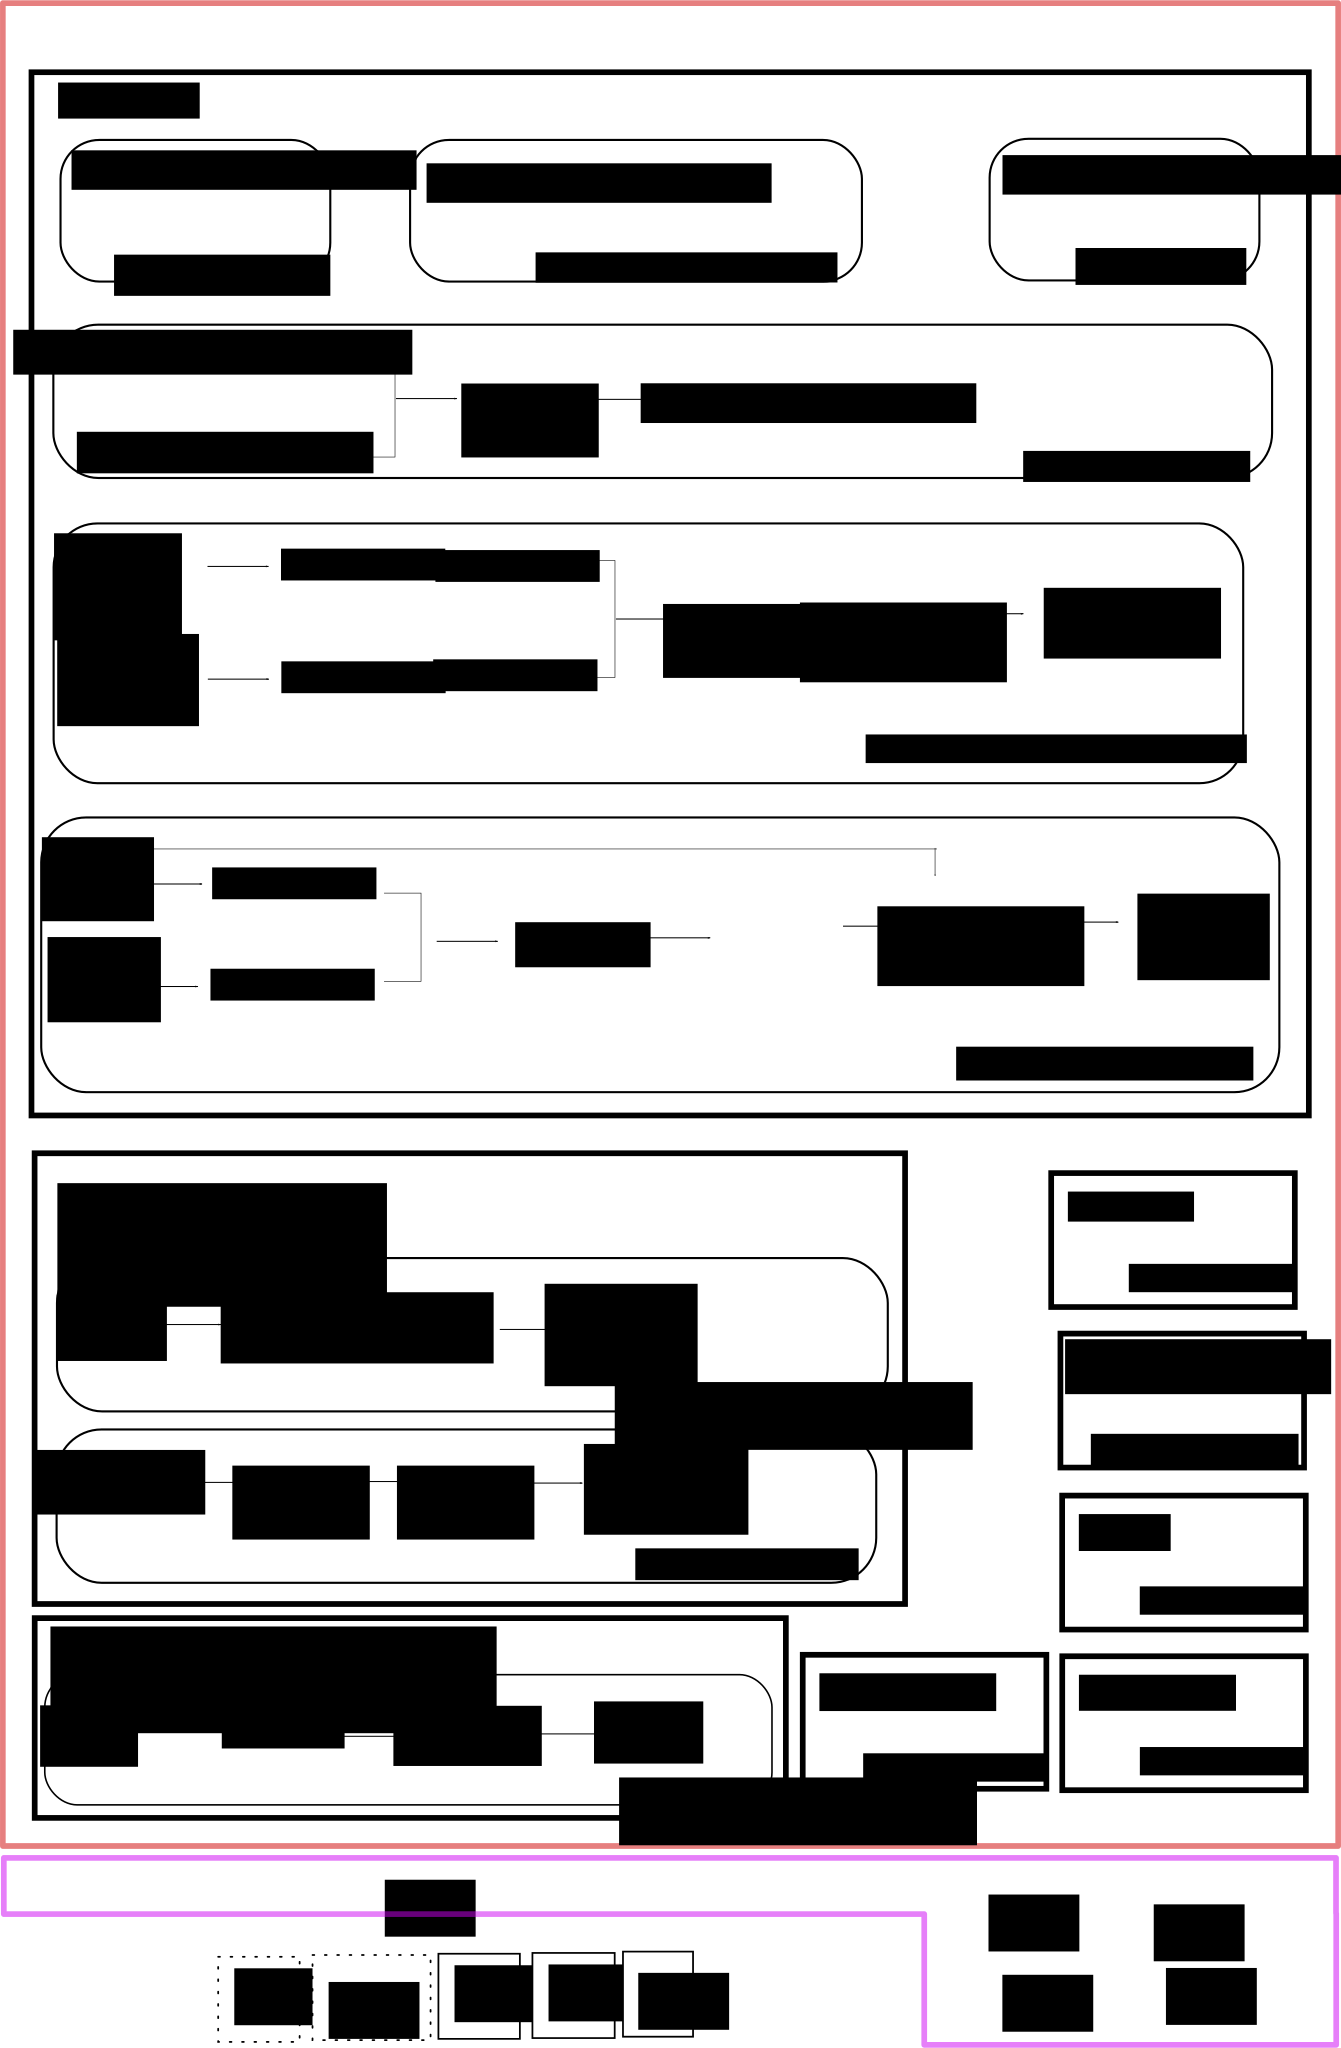
\includegraphics[width=85mm]{dependencies}
\end{center}
\caption{\hl{Sammba-MRI major modules.}}\label{fig:architecture}
\end{figure}

\subsection{DICOM to NIfTI conversion}
Sammba-MRI allows to convert Bruker DICOM (digital imaging and communications in medicine) files to the standard  Neuroimaging Informatics Technology Initiative  format (NIfTI-1) and extracts extensive information using DCMTK package  \citep{eichelberg2004ten}. 
Bruker files conversion is an active development field,
with various available tools handling DICOM (e.g. 
dicomifier\footnote{\url{https://github.com/lamyj/dicomifier}}) or
not (e.g. bru2nii\footnote{\url{https://github.com/neurolabusc/Bru2Nii}},
Bruker2nifti\footnote{\url{https://github.com/CristinaChavarrias/Bruker2nifti}}, bruker2nifti\footnote{\url{https://github.com/SebastianoF/bruker2nifti}}).
Finally, ParaVision 360 with the latest patch 1.1 can export the NIFTI format since February 2019.
Our implementation is meant to be a light helper function, allowing to 
handle the conversion on the fly. It has been tested only for Paravision 6
and a limited number of imaging sequences.

\subsection{Bias field correction}
Intensity non-uniformity modelling is essential in preclinical studies
because the intensity gradient corrupting MR images becomes
particularly pronounced at high field strengths \citep{boyes2008intensity}.
Sammba-MRI relies on AFNI's \bashinline{3dUnifize} to correct for intensity bias in
anatomical images, and on \bashinline{N4BiasFieldCorrection} function
of the ANTs package \citep{tustison2010n4itk}
for the other modalities. 3dUnifize is also used to aid brain extraction,
as detailed in the following paragraph.

\subsection{Skull-stripping}
Skull-stripping is the critical early step in processing
MRI images from small animals. Various automatic rodent-specific 
software\Ccancel{s} \citep{chou2011robust, oguz2014rats} or adaptations of human algorithms (\citeauthor{wood2013rbet}, \citeyear{wood2013rbet}; AFNI's 3dskullstrip -rat)
are freely available for research purposes. We choose to rely on
the LOGISMOS-based graph segmentation \citep{yin2010logimos} based on grayscale mathematical morphology 
RATS software  \citep{oguz2014rats} because
of its good performance across a wide range of datasets \citep{sargolzaei2018comparative}.
An alternative to the free but non-open source RATS tool is also 
available, based on an adaptation of the 
human histogram-based brain extraction method of Nilearn. 
This method can be used in any pipeline by setting the parameter
 \pythoninline{use_rats_tool} to \pythoninline{False}.
Because intensity inhomogeneity can hamper the performance of automatic skull stripping,
prior bias field correction
is usually recommended \citep{sled1998nonparametric} and is performed by default with \bashinline{3dUnifize}.
The helper function \pythoninline{brain_segmentation_report}
from Sammba-MRI \pythoninline{segmentation} module allows to
efficiently tune the initial intensity threshold used in bias correction by
producing for a given set of thresholds 5 informative measures
characterizing the extracted mask to bypass 
time consuming repetitive visual checks.
The returned features consist of the total volume of
the extracted mask, its 
anteroposterior length, its right-left width, and its inferior-superior hight as well
as the sample Pearson's product-moment correlation
coefficient between the brain mask image and its reflection
with respect to the estimated mid-sagittal plane
\citep{powell2016fully}.

\section{Ready-to-use pipelines}

Sammba-MRI proposes optimized pipelines to perform spatial registration
to a population or standard reference template, inter-modalities
registration and functional and perfusion MRI processing.
State-of-the-art small animal registration pipelines available as FOSS
are the Atlas-based Imaging Data Analysis of structural and functional mouse
brain MRI (AIDAmri) \citep{pallast2019processing} package for the registration of functional and diffusion
mouse brain MRI with the Allen Brain Reference atlas and
the mouse-brain-optimized registration workflow \citep{ioanas2019optimized}
part of SAMRI package. 
Sammba-MRI pipelines have been tested throughout the different stages of their
development process on various datasets from mouse, rat and mouse lemur
and used in several publications from our lab \citep{garin2018resting, nadkarni20193d, garin2019resting}.
All pipelines start with bias filed correction for the individual images.
The registration itself relies on AFNI's \bashinline{3dAllineate} and \bashinline{3dQwarp} functions to 
estimate linear and nonlinear (piecewise polynomial $C^1$ diffeomorphism) transforms respectively between the source image
and the reference image. Internal parameters of these functions have been optimized for
small animal brains.
We experienced a better performance when linear registration
is performed on brain extracted images and nonlinear warps are computed
using whole head images, and therefore followed this strategy across all the 
registration pipelines.

\subsection{Template matching}
Template matching is a necessary step for group studies. Several reference
templates exist both for mouse and rat brains and the user needs to 
specify the path to the template of his choice to the \pythoninline{TemplateRegistrator}
class from the \pythoninline{registration} module.
\begin{minted}[
frame=single,
framesep=2mm,
baselinestretch=1.2,
fontsize=\scriptsize,
]{python}
from sammba.registration import 
    TemplateRegistrator
registrator = TemplateRegistrator(
    'dorr_t2.nii.gz',
    brain_volume=400)
registrator.fit('mouse01_t1.nii.gz')
\end{minted}
We evaluated the registration accuracy of the proposed pipeline  on 
the publicly available Brookhaven in vivo dataset, consisting of 
T2-weighted images of 12 C57BL/6J male adult mice and
their segmentations in 20 brain regions \citep{ma2008vivo}. The scans were 
acquired using a 9.4 T Bruker scanner at 100 \textmu m isotropic resolution. The 
public dataset had incomplete files/segmentations for 2 subjects so the evaluation was 
limited to 10 subjects.
Because the shared individual images have been pre-registered to one reference image, 
we submitted them to slight random quadratic deformations (Normally 
distributed coefficients with std=$0.1$ mm for translation, $0.1$ degrees for 
rotation, $0.02$ mm for scaling, $0.02$ mm for shear and $0.005$ mm for the remaining $31$ polynomial coefficients) before performing the registration to the template.
We then measured the regional overlap
between each region in the average atlas and the transformed mice atlases 
using Dice similarity coefficient ($2\frac{|A \cap B|}{|A| + |B|}$) .
For comparison purposes, the registration was also performed using SPM mouse \citep{sawiak2009spmmouse}.
Figure ~\ref{fig:dices} shows that Sammba-MRI pipeline achieves
high overlap values and outperforms SPM mouse in the majority of cases.
\begin{figure}[h!]
\begin{center}
\includegraphics[width=85mm]{rois_on_template}
\end{center}
\caption{Registration to template of 10 C57 mice: \textbf{(A)} individual mouse anatomical image registered 
to the template with 
the contours of the average atlas superimposed as coloured lines; \textbf{(B)} Dice  
coefficient between each region in the average atlas and the transformed mice atlases 
(per region and animal).}\label{fig:dices}
\end{figure}

\subsection{Group-wise registration}
Group-wise registration aims to align all images within a common
space, resulting in an average brain that represents the commonalities among
individual brain anatomies of a particular population.
The use of cohort-specific templates eliminates possible bias toward external
features and improves subsequent analyzes \citep{de2019towards}.
Sammba-MRI implements the multi-level, iterative scheme proposed by \citep{kovavcevic2005three}
to create a fine anatomical 
template from individual structural MRI scans. A first rough template is obtained
by averaging bias corrected head images centred on their respective brain masks \st{barycentres} \hl{centroid}. Then the individual images are registered to this template.
This process of successive averaging/registration is iterated while increasing the number of degrees of 
freedom of the estimated transform and updating the target template (see \citep{nadkarni20193d} for a detailed description of the pipeline).
The method adapts to different small animal species, e.g. mouse lemurs
\citep{nadkarni2018digital}, and allows the creation of high quality
group average templates (Figure ~\ref{fig:mouse_template}).
\begin{figure}[h!]
\begin{center}
\includegraphics[width=85mm]{mouselemur_template}
\end{center}
\caption{Mouse lemur template from 34 animals.}\label{fig:mouse_template}
\end{figure}

\subsection{Multi-modal processing}
In the context of the increasing use of multimodal imaging, several
MRI techniques can 
be acquired from small animals, including
structural imaging with different contrasts, 
blood-oxygenation-level-dependent (BOLD) and  arterial spin labeling (ASL) MRI.
In addition to the inherent difficulties in intermodality registration \citep{ashburner1997multimodal},
severe image artifacts can corrupt the non anatomical scan
resulting in a low signal-to-noise ratio (SNR).
For instance, the echo 
planar imaging (EPI) 
technique widely used in  
functional MRI and perfusion imaging
suffers nonlinear geometric and intensity distortions caused by static magnetic field 
inhomogeneity that 
worsen at higher field strengths and have a more dramatic impact on small brains
\citep{hong2015evaluation}. 

Intra-subject registration between an anatomical scan and another modality
is handled through the \pythoninline{Coregistrator} class from the
\pythoninline{registration} module. 
\begin{minted}[frame=single, framesep=2mm, baselinestretch=1.2,
fontsize=\scriptsize,]{python}
from sammba.registration import 
    Coregistrator
coregistrator = Coregistrator(
    brain volume =400)
\end{minted}

\subsubsection{Rigid-body registration}
Since orientation is correctly handled through the DICOM to NIfTI conversion,
the anatomical image is first reoriented to match the modality of interest.
Both images then undergo intensity unifization and brain extraction.
A rigid body
transform that minimizes normalized mutual information
between the brain extracted images is finally estimated and applied to the whole head images.
\begin{minted}[frame=single, framesep=2mm, baselinestretch=1.2,
fontsize=\scriptsize,]{python}
coregistrator.fit_anat(
    'mouse01_t1.nii.gz')
coregistrator.fit_modality(
    'mouse01_t2.nii.gz')
\end{minted}

\subsubsection{Reorientation-only}
It is possible that the source or/and the reference
images are of insufficient quality to correctly estimate a rigid body transform. In 
this case,
assuming that the head motion between the two acquisitions is low, it is better
to only reorient the anatomical image to match the modality of interest.
\begin{minted}[frame=single, framesep=2mm, baselinestretch=1.2,
fontsize=\scriptsize,]{python}
coregistrator.fit_anat(
    'mouse01_t1.nii.gz')
coregistrator.fit_modality(
    'mouse01_t2.nii.gz',
    reorient_only=True)
\end{minted}

\subsubsection{Resting state BOLD fMRI processing}
BOLD scans are preprocessed using the same usual steps for human data
with optional slice timing correction, bias field correction, realignment to the 
first volume
and computation of the temporal mean of all the volumes.
The corresponding structural scan is then registered to the average BOLD scan.
Since this is a critical step, the user can choose
either to pursue with human-like pipeline by estimating a rigid body functional-to-
structural transform and applying its inverse to the structural image, or to assume 
that the head motion between the two scans is negligible.
In all cases, the transformed or not structural image is then reoriented
to match the functional image. Next, the average functional image and the reoriented 
structural image are split into 2D slices along the z-direction (according to the 
slice geometry of the functional image) and each functional slice undergoes 
afterwards a nonlinear registration step to best match the corresponding structural 
slice. This per-slice registration corrects for EPI distortion while being more 
conservative than a global 3D nonlinear registration, to better manage large slice 
thickness in the BOLD acquisitions of small animals. Since geometric distortions are 
higher in the through plane direction due to the typically lower resolution than in-
plane, the correction is still satisfactory.

\subsubsection{ASL fMRI processing}
ASL is an attractive method 
to image the vascular system by directly measuring blood flow.
However, estimating the cerebral blood flow (CBF) in small animals is challenging due 
to the low SNR and lack of sensitivity \citep{kober2008experimental}.
Sammba-MRI allows to preprocess functional ASL scans with the M0 scan used 
as the representative volume for registration. 
No between volume realignment is performed because of the usual poor SNR.
For Bruker-FAIR (Flow-sensitive Alternating Inversion Recovery) EPI sequences,
quantitative   CBF   maps can be estimated using \pythoninline{fair_to_proc} 
function from the \pythoninline{modality_processor} module.

\subsection{Modality to template and vice versa}
BOLD and ASL preprocessing can be performed in the individual space with
\pythoninline{Coregistrator} or in template space with \pythoninline{TemplateRegistrator}.
In the latter case, the structural-to-template warp, the functional-to-structural 
rigid body transform and the perslice functional-to-structural warps are  
combined 
 and applied in a one-big-step transformation
to the functional data to minimize interpolation errors.
The \pythoninline{TemplateRegistrator} class encompasses an
\pythoninline{inverse_transform_towards_modality}
method to bring an image from the reference space to the individual's space.

\subsection{Results}
Resting state fMRI allows to study temporally synchronized BOLD oscillations
reflecting functionally connected brain networks.
As in human resting state fMRI, spatial networks can be extracted using Independent Components Analysis (ICA) 
and were successfully demonstrated in anaesthetized mice \citep{zerbi2015mapping, grandjean2019common}. 
We preprocessed the publicly shared functional data
from 15 mice (2-3 months old) from \citet{zerbi2015mapping} paper with Sammba-MRI and performed a group ICA 
\citep{varoquaux2010group} with 30 components. Relevant bilateral
regions related to
somatosensory, hippocampal, visual, basal ganglia,
and sensorimotor networks. 
were obtained without additional data post-processing Figure ~\ref{fig:ica}.
\begin{figure}[h!]
\begin{center}
\includegraphics[width=85mm]{{ica}}
\end{center}
\caption{ICA bilateral components. IC 1: Barrel field (i) cortex,
IC 5: Lateral striatum, IC 9: Dorsal striatum (i),
IC 10: Visual cortex, IC1 3: Hippocampus,
IC 16: Dorsal striatum (ii), IC 17:   Barrel field (ii) cortex,
IC 21: Ventral striatum, IC 26: Supplementary cortex}
\label{fig:ica}
\end{figure}
To illustrate the perfusion processing pipeline, we used perfusion FAIR images from 10 C57BL/6J mice (5-7 months)
to quantify CBF.
Figure ~\ref{fig:cbf} shows voxelwise map averaged across all individuals and regional absolute CBF values, all 
in agreement with the literature \citep{muir2008cerebral}.
%Our implementation processes 10 mice, more than 300Gb, in only 20 minutes (regular desktop, 8Gb of RAM) [1 mice with 30 volumes, resolution, number of slices etc].
\begin{figure}[h!]
\begin{center}
\includegraphics[width=85mm]{cbf}
\end{center}
\caption{CBF from 10 C57 mice in ml/100g/min:  \textbf{(A)} group   average   CBF   map ;  \textbf{(B)} individual regional CBF.}\label{fig:cbf}
\end{figure}
\section{Big data, reproducibility, collaboration}
The package design facilitates big data exploration: the user is able to run an 
entire analysis in a single Python script, rerunning pipelines is optimized 
through Nipype caching mechanism and long lasting steps (nonlinear warping, perfusion 
fitting) are executed in parallel.
We believe that reproducibility in the neuroimaging field is not possible without
making the acquired images and the preprocessing code available to the community.
For this reason, Sammba-MRI promotes the sharing of MRI data by providing 
utility functions to download public small animal brain MRI 
datasets and relies on it for demoing the package capabilities.
In order to encourage external contributions, our library source code is hosted on the open 
collaborative GitHub platform
and distributed under the CeCILL v2.1 license, a FOSS license adapted to both international and French legal matters 
allowing anyone to make changes and redistribute it. 
Sammba-MRI supports GNU/Linux and Mac OS X operating systems (OS), used by over 70\% 
of neuroimagers \citep{hanke2011neuroscience}. 

\section{Conclusion}

By efficiently combining different existing human and animal neuroimaging
tools, Sammba-MRI allows to tackle common processing issues in a fully
automated fashion. High quality spatial registration can be easily performed, 
including template matching, between modalities registration as well as
the creation of cohort-specific templates. Sammba-MRI also implements
functional and perfusion MRI preprocessing methods and cerebral blood flow
estimation for FLAIR perfusion images. Emphasis is put on code readability
and ease of use to favour contributions from the community.

\section*{Conflict of Interest Statement}

The authors declare that the research was conducted in the absence
of any commercial or financial relationships that could be construed
as a potential conflict of interest.

\section*{Author Contributions}

SB, NN and MC contributed code to the project. NN, CG and MD contributed
to data acquisition. SB wrote the manuscript with input from CG and NN.
Every author read and approved the manuscript.

\section*{Funding}

We thank the France-Alzheimer Association, Plan Alzheimer Foundation
and the French Public Investment Bank's "ROMANE" program for funding this study.

\section*{Data Availability Statement}

The mouse lemur dataset can be automatically loaded through Sammba-MRI or
directly from \url{https://nitrc.org/projects/mouselemuratlas} for the template
and \url{https://openneuro.org/datasets/ds001945} for the original anatomical images. The perfusion
dataset will be made publicly available following publication.

\bibliographystyle{frontiersinSCNS_ENG_HUMS} 

\bibliography{sammba}

\end{document}
